\documentclass[10pt]{article}   	% use "amsart" instead of "article" for AMSLaTeX format

%\geometry{landscape}                		% Activate for rotated page geometry
%\usepackage[parfill]{parskip}    		% Activate to begin paragraphs with an empty line rather than an indent
%\usepackage{graphicx}				% Use pdf, png, jpg, or eps§ with pdflatex; use eps in DVI mode
								% TeX will automatically convert eps --> pdf in pdflatex		
\usepackage{amssymb}
\usepackage[cm]{fullpage}
\usepackage{tabularx}
\usepackage{float}
\usepackage{amsmath}
\usepackage{algorithmic}
\usepackage[hypcap]{caption}
\usepackage{graphicx}
\usepackage{framed}
\usepackage{subfigure}
\usepackage[titletoc,toc,title]{appendix}
\usepackage{listings}

%\floatstyle{boxed}
\restylefloat{figure}

\lstset{language=Matlab,%
    %basicstyle=\color{red},
    breaklines=true,%
    morekeywords={matlab2tikz},
   % keywordstyle=\color{blue},%
    %morekeywords=[2]{1}, keywordstyle=[2]{\color{black}},
 %   identifierstyle=\color{black},%
  %  stringstyle=\color{mylilas},
  %  commentstyle=\color{mygreen},%
 %   showstringspaces=false,%without this there will be a symbol in the places where there is a space
  %  numbers=left,%
    %numberstyle={\tiny \color{black}},% size of the numbers
    numbersep=9pt, % this defines how far the numbers are from the text
  %  emph=[1]{for,end,break},emphstyle=[1]\color{red}, %some words to emphasise
    %emph=[2]{word1,word2}, emphstyle=[2]{style},    
}

\title{
	Machine Learning and Neural Computation\\
	\textbf{Assessed Coursework}
 }
\author{
	Beatriz Isabel Lopez Andrade (bil14)
}
%\date{}							% Activate to display a given date or no date

\begin{document}
\maketitle
\begin{abstract}
The present report assesses Monte-Carlo and Temporal Difference (specifically TD(0)) Reinforcement Learning methods on several Grid Worlds. This report discusses the implementation and the influence of different parameters on the performance of both methods.
\end{abstract}

\section*{Introduction}
One of the main properties of Monte-Carlo and Temporal Difference methods is that, unlike Dynamic Programming, they do not need a complete knowledge of the environment, instead they can learn from experience. In the case of Monte-Carlo methods, this experience is a set of complete traces, from an initial state to an absorbing one, formed by several tuples (action, state, reward), that describe each of the transitions. Temporal Difference also uses traces, but it does not need complete ones, since it partially relies on previous estimations to perform policy evaluation, i.e. it bootstraps. \cite{sutton}

This report is divided into two sections, namely sections A and B. The first one focuses on Monte-Carlo Reinforcement Learning Methods. In particular, it discusses First Visit Monte-Carlo, and the parameters that influence its performance. Section B discusses  the Temporal Difference method TD(0). The main aim of the last section is to analyze the performance of the Temporal Difference  policy control method Sarsa on two different Grid Worlds. 

\section*{Section A}

This section briefly describes the implementation of \textbf{First-Visit Monte Carlo} and evaluates the performance of Monte-Carlo Batch optimization on \texttt{GrindWorld1}. In particular, estimates the number of traces needed to compute an accurate state-action value function (\^{Q}) and the number of batches until the optimal policy is found. It also discusses how the previous computations are affected by the discount factor ($\gamma$) and the exploration-exploitation factor ($\epsilon$), respectively.

In order to obtain the traces to perform Monte-Carlo and Temporal Difference estimations the function \texttt{GetTrace} is used. This function outputs a random episode from a given MDP. Each row in the output has three columns, that represent the reward for a transition from the previous state to the current one having taken a particular action, the current state, and the action taken in the current state to move to the following one.

In general, the function \texttt{GetTrace} generates a random sample of the current state taken into account the previous state and the chosen action in that state. After that, it gets the reward corresponding to that transition and action. If the current state is not an absorbing one, the function generates a random sample of the action in that state. On the contrary, if the current state is an absorbing one, none further actions are taken and therefore, the trace ends. The row corresponding to this state is formed by the reward, the state itself, and the action taken in the current state.

\begin{table}[!h] 
	\begin{center}
		\begin{tabular}{ | c c  c | }
		\hline
		Reward & Status & Action \\ \hline \hline
		0 & 4 & R \\ \hline
		-1 & 5 & R \\ \hline
		-1 & 6 & L \\ \hline
		1 & 5 & L \\ \hline
		1 & 4 & R \\ \hline
		-1 & 5 & R \\ \hline
		-1 & 6 & R \\ \hline
		10 & 7 & 0 \\ \hline
		\end{tabular}
		\caption{Trace corresponding to the Stair Climbing MDP.\label{tab:traceStair}}
		
	\end{center}
\end{table}

Table ~\ref{tab:traceStair} shows a sample trace of \textbf{Stair Climbing MDP} (Figure~\ref{stairClimb}), the first state is four, because the function \texttt{StairClimbingMDP} assigns a probability of one to this state as the first state. The action in this state is \texttt{Right}, but it could have been \texttt{Left}, as the unbiased policy is used. In the following row, the state is five, since the probability of going from state four to five having taken action \texttt{Right} is one. The reward for this transition is -1 and the next action \texttt{Right}, but it could have been \texttt{Left}. The following rows are computed in the same way, until an absorbing state is reached. In the case of the first row, there is no transition to get to the current state, i.e. it is the first state. Hence, there is no reward for getting to that particular state. That is the reason why a dummy value is assigned to the first reward. In an absorbing state, the state where the trace ends, no further actions are taken. Therefore, the value for the last action is a dummy one.

\begin{figure}[!h]
\centering
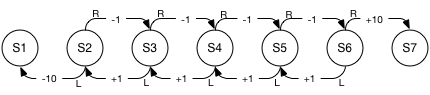
\includegraphics[scale=0.6]{./figures/StairClimbingMDP}
\caption{States, actions, and rewards in Stair Climbing World.\label{fig:stairMdp}}
\end{figure}

As stated before, Monte Carlo methods rely on experience. In this project, \texttt{GetTrace} generates the sample traces needed to compute an estimate of the action-value function \^{Q}, which is required to generate an approximation to the optimal policy using Monte Carlo policy control. The function \texttt{MonteCarloEstimation} implements \textbf{First-Visit Monte-Carlo} state-action value estimation. The implementation of this function is shown in procedural form in Figure~\ref{fig:mcfv}. The matrix of Q-values is estimated as the average of the returns following the first visit to each state-action for all the traces.
\begin{figure}[!ht]
\begin{framed}
\begin{algorithmic}
 	\STATE SumReturns(s,a) $\leftarrow$ 0, $\forall$ s $\in$ States, $\forall$ a $\in$ Actions\;
 	\STATE N(s,a) $\leftarrow$ 0, $\forall$ s $\in$ States, $\forall$ a $\in$ Actions\;
	 \FOR{$i=1$ \TO n}
  		\STATE generate a new trace\;
  		\IF{first time (s,a) appearing in the trace}
   			\STATE R $\leftarrow$ return following the first occurrence of (s,a)\;
   			\STATE SumReturns(s,a) $\leftarrow$ SumReturns(s,a) + R\;
   			\STATE N(s,a) $\leftarrow$ N(s,a) + 1\;
  		\ENDIF
 	 \ENDFOR
 \STATE Q(s,a) $\leftarrow$ SumReturns(s,a) / N(s,a), $\forall$ s $\in$ States, $\forall$ a $\in$ Actions\;
\end{algorithmic}
\end{framed}
 \caption{First-Visit Monte-Carlo implementation.\label{fig:mcfv}}
 \end{figure}
 
As said before, in Monte Carlo methods the interaction with the environment is essential. Hence, it is important to maintain a certain degree of exploration, otherwise we cannot ensure that all the actions are evaluated a reasonable amount of times and, therefore, the convergence to an approximation of the optimal policy ($\epsilon$-greedy policy) cannot be guaranteed. One of the approaches to tackle this issue is on-policy Monte Carlo control. In general, this method generates \textit{soft} policies, where all the actions have a certain probability, even the non-optimal ones. As a consequence, these kind of policies cannot be optimal, however when converging, they can be good approximations of the optimal one. Apart from \texttt{MonteCarloEstimation}, two other functions, \texttt{eGreedyPolicyFromQ} and \texttt{MonteCarloBatchOptimisation}, were developed to implement on-policy Monte Carlo control.

The function \texttt{eGreedyPolicyFromQ} outputs an $\epsilon$-greedy policy based on the state-action value function. The function \texttt{MonteCarloBatchOptimisation} implements on-policy Monte-Carlo Batch optimisation, where \^{Q} and $\epsilon$-greedy policy are updated in each batch, with the aim of improving the policy. 

\begin{figure}[!h]
\centering
\setlength\fboxsep{0pt}
\setlength\fboxrule{0.6pt}
\fbox{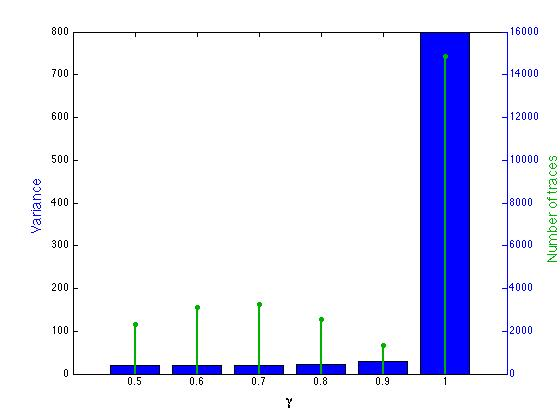
\includegraphics[scale=0.5]{./figures/fig_maximum_variance}}
\caption{Mean of the maximum variance of 20 different Q estimations and corresponding mean of the number of sample traces needed to converge to an accurate Q estimation for different values of $\gamma$. \label{fig:maxvar}}
\end{figure}

On-policy Monte-Carlo control was applied on \texttt{GridWorld1}. The rest of the section focus on the selection of the number of sample traces, $\gamma$, the number of batches, and $\epsilon$ for this particular environment. First, our findings about the relation between the number of traces and $\gamma$, as well as the values chosen for these two parameters are discussed. After that, we talk about the values of $\epsilon$ and the number of batches, and how they impact the performance of on-policy Monte Carlo control.

\texttt{MonteCarloBatchOptimisation} obtains the policy from the state-action value function, therefore the estimation \^{Q} must be accurate. As the number of traces tends to infinity, the estimate \^{Q}  converges to its real value. In practice, however, the number of traces must be finite and, ideally, should be a small. It is important to notice that the quantity of sample traces required not only depends on the complexity of the networks and the sample traces themselves, but the discount factor $\gamma$ also influence it.

In order to evaluate the impact of $\gamma$ on the convergence of the estimation, the function \texttt{MonteCarloEstimationTestn} was created. It implements Monte-Carlo state-action value estimation (like \texttt{MonteCarloEstimation}) with on-line averaging.\footnote{ For each new sample: \begin{algorithmic}
  \STATE Q(s,a) $\leftarrow$ Q(s,a) + (R - Q(s,a)) / N(s,a), $\forall$ s $\in$ States, $\forall$ a $\in$ Actions\;
\end{algorithmic}} This function outputs the estimation of the state-action value function, the number of sample traces needed to converge with an accuracy level of 0.001 given a particular set of random traces, and the maximum value of the variance of the returns for each state and action. 

Figure~\ref{fig:maxvar} shows the mean of the maximum variance of the state-action value function estimation for 20 trials and the corresponding mean of the number of sample traces required to converge for different values of the discount factor $\gamma$ (from 0.5 to 1). The figure suggests that if the variance is high, the number of traces needed to converge is also high; this is the case when $\gamma$=1, i.e. no \textit{discounting} is applied in the calculation of the return. It is important to notice that the sample traces can be arbitrarily long (they may include multiple loops). The return of traces with a high number of steps is prone to have a high absolute value, which may differ significantly from the returns of shorter traces; causing a high variance.\footnote{This values are computed assuming that S8 is the initial state.}

\begin{figure}[ht!]
     \begin{center}
%
        \subfigure[Greedy Policy for $\gamma$=0.5]{%
            \label{fig:firsta}
            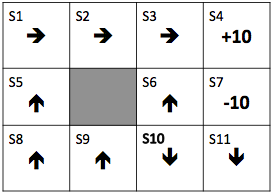
\includegraphics[scale=0.45]{./figures/gamma_05}
        }%
        \subfigure[Greedy Policy for $\gamma$=0.6]{%
           \label{fig:seconda}
           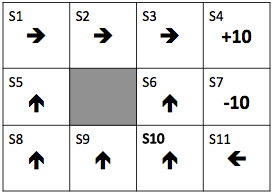
\includegraphics[scale=0.45]{./figures/gamma_06}
        }%
         \subfigure[Optimal Policy]{%
            \label{fig:thirdA}
            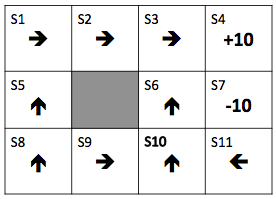
\includegraphics[scale=0.45]{./figures/optimal_policy}
        }%
        %
    \end{center}
    \caption{%
        Actions with the highest probabilities in the $\epsilon$-greedy policies computed using Monte-Carlo Batch optimization for $\gamma$ between 0.5 and 1, and $\epsilon=0.5$. 
     }%
   \label{fig:gammacomp}
\end{figure}

From the previous results, the discount factor is concluded to be less than 1. It is important to notice, however, that when $\gamma$ is too low, the return maximizes immediate rewards. In this scenario, actions taken to maximize returns in states "far" from the goal may decrease the chances to get to the final goal, where the reward is high. This leads to the inability of selecting global optimal actions from the state-action value function. Figure~\ref{fig:gammacomp} shows the action with the highest probability in each state as computed by the function \texttt{MonteCarloBatchOptimasation} when $\epsilon=0.5$. When $\gamma$=0.5, the preferred actions in S9, S10, and S11 do not lead to S4 (absorbing state with the highest reward); this also happens in S9 when $\gamma$=0.6. On the contrary, for higher values of $\gamma$, \texttt{MonteCarloBatchOptimasation} assigns the highest probability to optimal actions when the number of batches N is sufficiently large and the state-action value function estimates are accurate.

As Figure~\ref{fig:maxvar} suggests, the mean number of sample traces needed to compute  \^{Q} with an accuracy level of 0.001 does not vary much for $\gamma$ between 0.5 and 0.9. Therefore, the value of the \textbf{discount factor $\gamma$} chosen is \textbf{0.9}, to ensure that the optimal actions have the highest probability in the $\epsilon$-greedy policy (obtained by calling the function \texttt{MonteCarloBatchOptimasation}). The \textbf{number of traces n}, in this case, is \textbf{2042}, which is an estimation of the maximum number of sample traces required to compute  \^{Q} with an accuracy level of 0.001.

\begin{figure}
\centering
\setlength\fboxsep{0pt}
\setlength\fboxrule{0.5pt}
\fbox{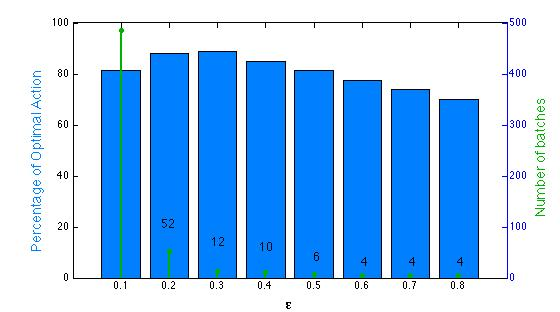
\includegraphics[scale=0.6]{./figures/epsilonfig}}
\caption{Percentage of optimal actions in  $\epsilon$-greedy policies  and estimation of the maximum number of batches to converge to a good approximation of the optimal policy for different values of $\epsilon$. \label{fig:epsilon}}
\end{figure}

When searching for the optimal policy using Monte-Carlo methods, it is important to maintain the appropriate balance between exploration and exploitation. If what seems the best choice is always followed, then other possible better options are not explored, and the optimal policy is never found. If, on the contrary, other alternative actions are also tested, the algorithm is prone to discover better choices. However, a  fixed exploration factor makes impossible to achieve an optimal policy, since all the actions have a certain probability.

Once the number of sample traces \texttt{n} and the discount factor $\gamma$ are settled, appropriate values for the number of batches \texttt{N} and the exploration-exploitation factor must be established. As stated before, these two parameters are crucial to converge to a good approximation of the optimal policy. In order to compute them, the function \texttt{MonteCarloBatchOptimasationTestN} is used. This function iterates until it converges to a final $\epsilon$-greedy policy. Figure~\ref{fig:epsilon} shows the maximum number of batches computed for different values of $\epsilon$ taken into account 20 trials. It also displays the percentage of optimal actions in the $\epsilon$-greedy policies computed by \texttt{MonteCarloBatchOptimasation} for the maximum number of batches obtained previously and the corresponding $\epsilon$.

As Figure~\ref{fig:epsilon} suggests, for small values of $\epsilon$ the number of batches to converge to an $\epsilon$-greedy policy is quite high compared to bigger values of this parameter. This is because methods with high $\epsilon$ explore more and, therefore, find the optimal actions faster. However, they assign a high probability to non-optimal actions. Hence, in general the percentage of optimal actions for this methods is lower than for methods with a small $\epsilon$, when policy convergence is reached.

It is important to notice that when the exploration is low, optimal actions are not always identified. On the contrary, if it is high, the optimal actions are detected, assuming a sufficiently large number of batches and accurate estimation of Q. However, the probability of each action is assigned taken into account not only the state-action value function, but also the exploration-exploitation factor, so that all the actions have a certain probability. As suggested by \cite{sutton}, a good approach could be decrease the value $\epsilon$ over the time, so it could converge to the optimal policy. For the particular \texttt{GridWorld1}, the value of the parameter \textbf{ exploration-exploitation factor $\epsilon$} chosen is \textbf{0.3} and the \textbf{number of batches \texttt{N}, 12}; since the method generates a policy with a high percentage of optimal values (88.75$\%$) for a fairly low maximum number of batches (12), and the optimal actions were correctly identified.

Table~\ref{tab:parameters} summarizes the parameters chosen when applying the function \texttt{MonteCarloBatchOptimasation} on \texttt{GridWorld1}.

\begin{table}[!h] 
	\begin{center}
		\begin{tabular}{ | c c  | }
		\hline
		gamma & 0.9 \\ \hline
		n & 2042\\ \hline
		epsilon & 0.3 \\ \hline
		N &  12\\ \hline
		\end{tabular}
		\caption{Choice of parameters for \texttt{MonteCarloBatchOptimasation} on \texttt{GridWorld1}.\label{tab:parameters}}
		
	\end{center}
\end{table}

In the previous simulations, the initial state was deterministically \texttt{S8}. This should not affect the performance of \texttt{MonteCarloBatchOptimasation} when the exploration is fairly high, since all the states are likely to be visited a sufficiently large amount of times. On the contrary, for small values of $\epsilon$, the initial state may have a big impact. If the initial state is near the goal, states that are "far" from the latest are not visited as frequent as others. This leads to poor estimations of the state-action values for these particular states, and consequently, actions computed by the $\epsilon$-greedy policy are prone to be non-optimal in such states. 

\texttt{MonteCarloBatchOptimasation} was also run on the Stair Climb MDP (Figure~\ref{fig:stairMdp}). In this case, Monte Carlo Batch Optimisation generates a good approximation to the optimal policy, assigning the maximum probability to optimal actions in each of the states, using a fairly low amount of traces. The reason is that This environment is much simpler than the Grid World one, not only because the number of state and actions is lower, but also because the actions have deterministic effects.


\section*{Section B}

This section focuses on Temporal Difference TD(0) methods for policy evaluation and control. In particular, it tests the performance of Sarsa, the on-policy TD(0) control method. Temporal Difference methods are similar to the  Monte Carlo approach in the sense that both rely on interactions with the environment. However, Temporal Difference methods does not need complete episodes, instead they learn from each step. This is possible because they use estimations of the returns of future episodes, i.e. they \textit{bootstrap}.\cite{sutton}

Sarsa method was tested on two grid worlds: \texttt{GridWorld2} and \texttt{GridWorld3}. These environments were obtained by executing the corresponding Matlab functions, which output a set of parameters that fully describe them. \texttt{GridWorld2} has the same topology than \texttt{GridWorld1} used in Section A. It is important to notice that the transmission matrix is noisy, i.e. the actions does not have a deterministic effect, with probabilities {0.8,  0.1, 0.1, 0}. Unlike \texttt{GridWorld1}, in \texttt{GridWorld2} the reward of the absorbing state S7 is -100; all the other rewards are -1, except from the one corresponding to the absorbing state S4, which is +10. The initial state is deterministically S8. The most relevant features are represented in Figure~\ref{fig:gridWorld23_a}.

\texttt{GridWorld3} consists of 22 states. The possible actions are {N, E, S, W}, as in the other two Grid Worlds. In this case, the transition matrix is also noisy, with the same probability distribution as before. The rest of the properties that define this world can be seen in Figure~\ref{fig:gridWorld23_b}. The function \texttt{DisplayGrid} can be used to display different parameters corresponding to each of the cells in the Grid Worlds.

\begin{figure}[ht!]
     \begin{center}
%
        \subfigure[Grid World 2 \label{fig:gridWorld23_a}]{%
            \label{fig:firstb}
            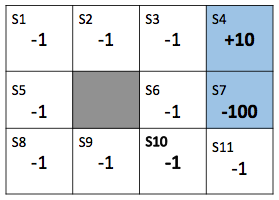
\includegraphics[scale=0.45]{./figures/GridWorld2}
        }%
        \subfigure[Grid World 3 \label{fig:gridWorld23_b}]{%
           \label{fig:secondb}
           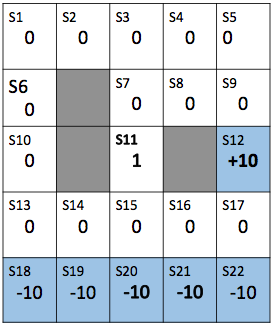
\includegraphics[scale=0.45]{./figures/GridWorld3}
        }\\ %  ------- End of the first row ----------------------%
       \end{center}
    \caption{%
       Names, rewards, and absorbing states (blue cells) corresponding to Grid World 2 and Grid World 3. 
     }%
   \label{fig:gridWorld23}
\end{figure}

Sarsa algorithm is the on-policy TD(0) control method. This method consists of two steps: first, it computes an approximation of the optimal state-action value function using TD(0); then, it generates the greedy policy from the previous approximation. It is important to notice that the estimation of the optimal policy is an iterative process, during which the value of  \^{Q} is updated in each considered step of the sample traces. In a similar way that Monte Carlo policy control, it is important to maintain a certain degree of exploration when computing  \^{Q}. Therefore, the actions are taken accordingly a $\epsilon$-greedy policy obtained from \^{Q}.

In order to analyze the performance of Sarsa, this algorithm was applied on \texttt{GridWorld2} and \texttt{GridWorld3}. Figure~\ref{fig:gw2op_a} shows the optimal policy for \texttt{GridWorld2}. This optimal policy was computed using Value Iteration, as it is guaranteed to converge to the optimal policy, for a sufficiently small accuracy level. Figure~\ref{fig:sarsaGrid2} displays the percentage of optimal actions taken by Sarsa. This values where computed using a discount factor $\gamma$=0.9 (for the reasons explained in Section A), exploration-exploitation factor $\epsilon$=0.01 (to introduce a small factor of exploration when estimating Q), learning rate $\alpha$=0.1 (to maintain a compromise between previous estimations and new knowledge), and maximum number of considered steps per trace maxsteps=20 (the length of the traces is usually below 20 when the unbiased policy is used) for different number of sample traces. Figure~\ref{fig:sarsaGrid2} suggests that for a sufficiently large amount of sample traces (about 150), Sarsa generates good approximations to the optimal policy, however, it is not able to converge to this one. From the data obtained during the simulation, it seems that the main problem is that Sarsa is not able to correctly identify the optimal action in S10.

In the case of \texttt{GridWorld3} this analysis is quite complex, since there are two optimal policies; state S11 has two optimal action: E and W (see Figure~\ref{fig:gw2op_b}). In this case, the discount factor $\gamma$ is 0.9; the learning rate $\alpha$, 0.1; the exploration-exploitation factor $\epsilon$, 0.1 (since the number of states is higher, we decide to increase this value to guarantee that all the states are visited a reasonable amount of times), the maximum number of considered steps per trace maxsteps is 100 (the length of the traces is usually below 100 when the unbiased policy is used). When the number of traces is low (below 10000), the estimation of the optimal state-action value function is very poor, since most of the state-action pairs are not evaluated a significant amount of times. This leads to the generation of policies that are far from the optimal ones. When more traces are considered (above 20000), the estimation of the optimal state-action value function is better. In this case, the policies obtained by Sarsa are good approximations of the optimal ones. However, this method does not converge to the optimal policies, as it seems to have difficulties identifying optimal actions mainly in the following estates: S3, S7, S11. 


\begin{figure}
\centering
\subfigure[Optimal Policy for Grid World 2 \label{fig:gw2op_a}]{%
	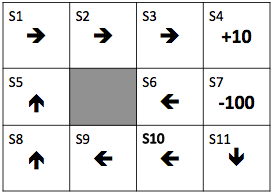
\includegraphics[scale=0.45]{./figures/GridWorld2OptimalPolicy}
}
\subfigure[Optimal Policies for Grid World 3 \label{fig:gw2op_b}]{%
	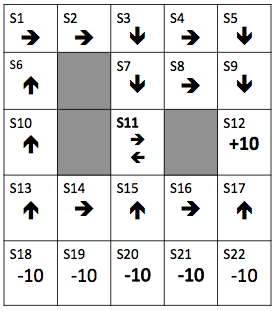
\includegraphics[scale=0.45]{./figures/GridWorld3OptimalPolicy}
} 
\caption{Optimal Policies for Grid World 2 and Grid World 3. \label{fig:gw2op}}
\end{figure}

\begin{figure}
\centering
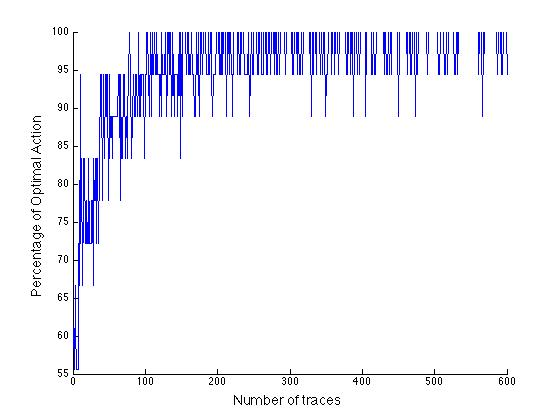
\includegraphics[scale=0.6]{./figures/SarsaGridWorld2}
\caption{Percentage of optimal actions in policies generated by Sarsa setting $\gamma$=0.9, $\epsilon$=0.01, $\alpha$=0.1, and maxsteps=20 for Grid World 2. \label{fig:sarsaGrid2}}
\end{figure}


\begin{appendices}
  \renewcommand\thetable{\thesection\arabic{table}}
  \renewcommand\thefigure{\thesection\arabic{figure}}
  \section{Source code} \label{app:newFunct}
  \subsection{\texttt{MonteCarloEstimation.m}}
  \begin{framed}
  \lstinputlisting{../MonteCarloEstimation.m}
  \end{framed}
  \subsection{\texttt{eGreedyPolicyFromQ.m}}
  \begin{framed}
  \lstinputlisting{../eGreedyPolicyFromQ.m}
  \end{framed}
  \subsection{\texttt{MonteCarloBatchOptimisation.m}}
  \begin{framed}
  \lstinputlisting{../MonteCarloBatchOptimisation.m}
  \end{framed}
   \subsection{\texttt{Sarsa.m}}
  \begin{framed}
  \lstinputlisting{../Sarsa.m}
  \end{framed}
\end{appendices}

\begin{thebibliography}{9}

\bibitem{sutton}
  Sutton, R. $\&$ Barto, A. (2005) \textit{Reinforcement Learning: An Introduction}, Cambridge, The MIT Press. 
  \bibitem{faisal}
  Faisal, A. (2014) \textit{Machine Learning $\&$ Neural Computation Lecture Notes}, London, Imperial College London. 
\end{thebibliography}


\end{document}  